\documentclass[a4paper]{article}
\usepackage{a4wide}
\usepackage{amsmath}
\usepackage{graphicx}
\usepackage{indentfirst}
% \usepackage[spanish]{babel}
\usepackage{amsfonts}
\usepackage{hyperref}

\usepackage[usenames,dvipsnames]{pstricks}
\usepackage{epsfig}
\usepackage{pst-grad} % For gradients
\usepackage{pst-plot} % For axes
\usepackage[space]{grffile} % For spaces in paths
\usepackage{etoolbox} % For spaces in paths
\makeatletter % For spaces in paths
\patchcmd\Gread@eps{\@inputcheck#1 }{\@inputcheck"#1"\relax}{}{}
\makeatother
\usepackage[abs]{overpic}
\setlength\unitlength{1mm}

\newcommand{\Z}{\mathbb{Z}}
\newcommand{\angstrom}{\textup{\AA}}

\renewcommand\contentsname{\'Indice}
\renewcommand\figurename{Figura}

\begin{document}
\title{Interfer\'ometros por divisi\'on de amplitud}
\author{P. Cobelli}
\date{Fecha de \'ultima actualizaci\'on: 14 de Noviembre de 2015}
\maketitle

\tableofcontents

\section{Acerca de este apunte}

Seg\'un vimos en las clases te\'oricas, en la experiencia de la doble rendija
de Young, del espejo de Lloyd, y en el biprisma de Fresnel (que emplearon en
el laboratorio), las ondas incidentes son {\bf divididas} mediante el uso de
rendijas, un espejo y un biprisma, respectivamente. Este m\'etodo de
divisi\'on, dijimos, se conoce como {\bf divisi\'on del frente de onda}. 
No obstante, seg\'un tambi\'en mencionamos, las ondas incidentes pueden 
dividirse tambi\'en \'opticamente por reflexi\'on, t\'ecnica que se conoce
como {\bf divisi\'on de amplitud}. Los interfer\'ometros que funcionan de 
acuerdo a este principio se denominan entonces {\it interfer\'ometros por
divisi\'on de amplitud}. En este apunte les ofrezco m\'as detalle acerca de 
este tipo de interfer\'ometros.

\section{Pel\'\i culas delgadas}

El primer ejemplo que consideraremos es el de un paquete de rayos de luz que
inciden sobre una pel\'\i cula delgada transparente, y que sufren reflexi\'on
(parcial) en las caras superior e inferior de la pel\'\i cula y viajan por
diferentes caminos, los cu\'ales pueden luego reunirse (por medio de una 
lente, por ejemplo) para producir interferencia. 

En principio, establezcamos una definici\'on. Decimos que una pel\'\i cula 
es {\bf delgada} cuando su espesor es de alrededor del orden de una 
longitud de onda de la luz visible que, por convenci\'on, podemos establecer
en 550 nm (5500 \angstrom). Esto implica que si el espesor de la pel\'\i cula
es de 50 $\mu$m, se la considera una pel\'\i cula gruesa. 

Una pel\'\i cula delgada puede ser una l\'amina delgada de un material 
transparente como vidrio o mica, pero tambi\'en puede estar compuesta por una
pel\'\i cula de aire encerrada entre dos placas transparentes, o incluso 
tratarse de la pared de una burbuja de jab\'on, seg\'un se muestra en la 
Fig.~\ref{fig:pompasjabon}.

Cuando la luz incide sobre una pel\'\i cula delgada, una porci\'on peque\~na 
de la luz se refleja en la superficie superior, mientras que la mayor parte
se transmite hacia el interior de la misma. Al viajar en la pel\'\i cula, 
una parte de la luz se refleja nuevamente hacia el interior de la pel\'\i cula
por la superficie inferior, y el resto termina emergiendo de la pel\'\i cula
hacia el medio exterior. Este funcionamiento se puede observar en el esquema
de la Fig.~\ref{fig:1}. 

\begin{figure}[ht]
    \centering
    \vspace{0.5cm}
    % 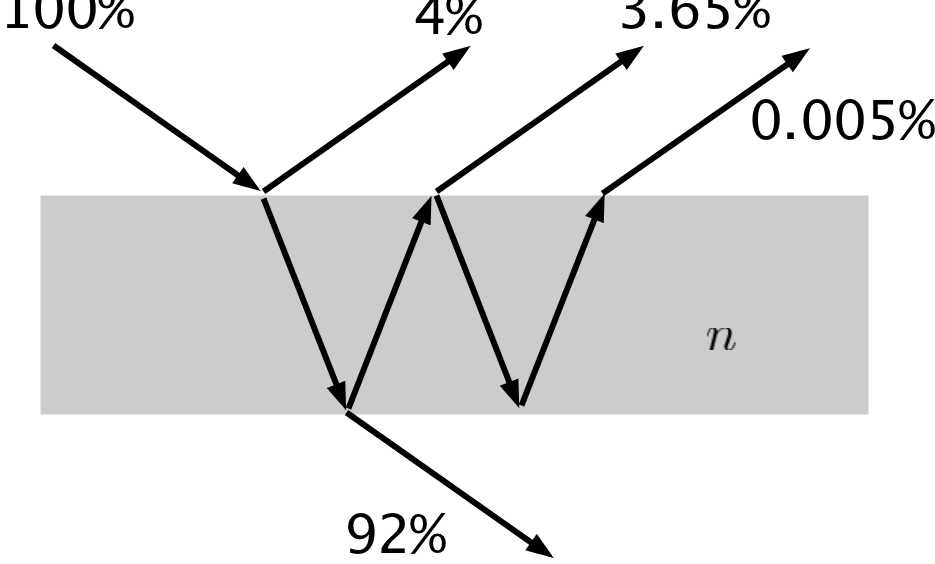
\includegraphics{rayos1.png}
    % \usepackage[usenames,dvipsnames]{pstricks}
% \usepackage{epsfig}
% \usepackage{pst-grad} % For gradients
% \usepackage{pst-plot} % For axes
% \usepackage[space]{grffile} % For spaces in paths
% \usepackage{etoolbox} % For spaces in paths
% \makeatletter % For spaces in paths
% \patchcmd\Gread@eps{\@inputcheck#1 }{\@inputcheck"#1"\relax}{}{}
% \makeatother
% % User Packages:
% 
% 
\psscalebox{1.0 1.0} % Change this value to rescale the drawing.
{
\begin{pspicture}(0,-1.8828238)(6.24,1.8828238)
\definecolor{colour0}{rgb}{0.8,0.8,0.8}
\psframe[linecolor=colour0, linewidth=0.04, fillstyle=solid,fillcolor=colour0, dimen=outer](5.792308,0.5823445)(0.2723077,-0.8776555)
\psline[linecolor=black, linewidth=0.04, arrowsize=0.05291667cm 2.0,arrowlength=1.4,arrowinset=0.0]{->}(0.35384616,1.5777291)(1.7384615,0.60849833)
\psline[linecolor=black, linewidth=0.04, arrowsize=0.05291667cm 2.0,arrowlength=1.4,arrowinset=0.0]{->}(1.7538462,0.5623445)(2.3076923,-0.8530401)
\psline[linecolor=black, linewidth=0.04, arrowsize=0.05291667cm 2.0,arrowlength=1.4,arrowinset=0.0]{->}(2.3076923,-0.8684247)(3.6923077,-1.8376555)
\psline[linecolor=black, linewidth=0.04, arrowsize=0.05291667cm 2.0,arrowlength=1.4,arrowinset=0.0]{<-}(3.1384616,1.5777291)(1.7538462,0.60849833)
\psline[linecolor=black, linewidth=0.04, arrowsize=0.05291667cm 2.0,arrowlength=1.4,arrowinset=0.0]{<-}(2.876923,0.5777291)(2.323077,-0.8376555)
\psline[linecolor=black, linewidth=0.04, arrowsize=0.05291667cm 2.0,arrowlength=1.4,arrowinset=0.0]{->}(2.9076922,0.5777291)(3.4615386,-0.8376555)
\psline[linecolor=black, linewidth=0.04, arrowsize=0.05291667cm 2.0,arrowlength=1.4,arrowinset=0.0]{<-}(4.0307693,0.5931137)(3.476923,-0.8222709)
\psline[linecolor=black, linewidth=0.04, arrowsize=0.05291667cm 2.0,arrowlength=1.4,arrowinset=0.0]{<-}(4.292308,1.5777291)(2.9076922,0.60849833)
\psline[linecolor=black, linewidth=0.04, arrowsize=0.05291667cm 2.0,arrowlength=1.4,arrowinset=0.0]{<-}(5.4,1.5623446)(4.0153847,0.5931137)
\rput[bl](2.7538462,1.6546522){$2\%$}
\rput[bl](4.123077,1.6854215){$1.92\%$}
\rput[bl](5.0,0.9469599){$0.008\%$}
\rput[bl](0.0,1.6854215){$100\%$}
\rput[bl](2.3076923,-1.8068863){$96\%$}
\rput[bl](4.707692,-0.45304012){$n$}
\end{pspicture}
}


    \caption{Reflexiones sucesivas en una l\'amina delgada de caras paralelas
        compuesta de jab\'on con \'\i ndice de refracci\'on $n = 1.333$. 
        Los valores asociados a cada rayo corresponden a las intensidades 
        relativas porcentuales de las reflexiones sucesivas 
        en la pel\'\i cula delgada.}
        \label{fig:1}
\end{figure}




En el caso de pel\'\i culas delgadas transparentes, las interfaces superior
e inferior tienen el efecto principal de transmitir la luz incidente, y s\'olo 
la reflejan d\'ebilmente (en t\'erminos de intensidad). En estos casos, s\'olo
la primera reflexi\'on en la superficie superior y la primera reflexi\'on en
la superficie inferior ser\'an de intensidad apreciable. Como ejemplo podemos
considerar una burbuja de jab\'on, de \'\i ndice de refracci\'on 1.333. 
Seg\'un vieron en F\'\i sica I, la reflectividad $\mathcal{R}$ de la superficie superior 
de esta pel\'\i cula delgada hecha de jab\'on viene dada por:
\begin{equation}
    \mathcal{R} = \left( \frac{n_\text{jab\'on}-n_\text{aire}}
    {n_\text{jab\'on}+n_\text{aire}} \right)^2 =  
    \left( \frac{1.333-1}{1.333+1} \right)^2 = \frac{0.111}{5.443} = 0.02 .
\end{equation}
Esto significa que alrededor del 2\% de la luz incidente se refleja en la 
superficie de la burbuja de jab\'on; el resto se transmite al interior de ella.
Luego de dos reflexiones sucesivas, la intensidad reflejada ser\'a de 
$(0.02 \times 0.02) = 0.04$ \% de la intensidad inicial. Por esta raz\'on, 
solo consideraremos los primeros dos rayos. 

\begin{figure}
\centering
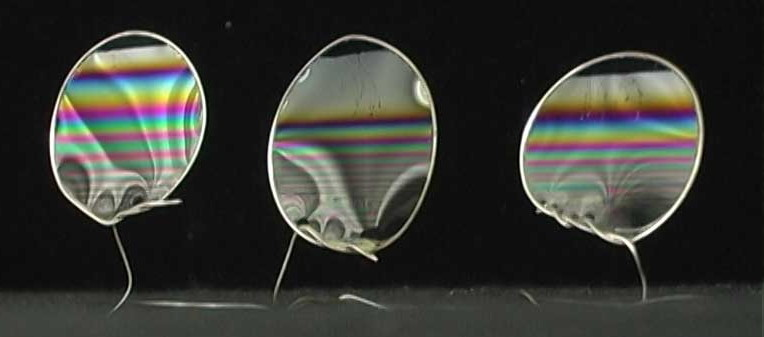
\includegraphics[height=5cm]{int_2.jpg}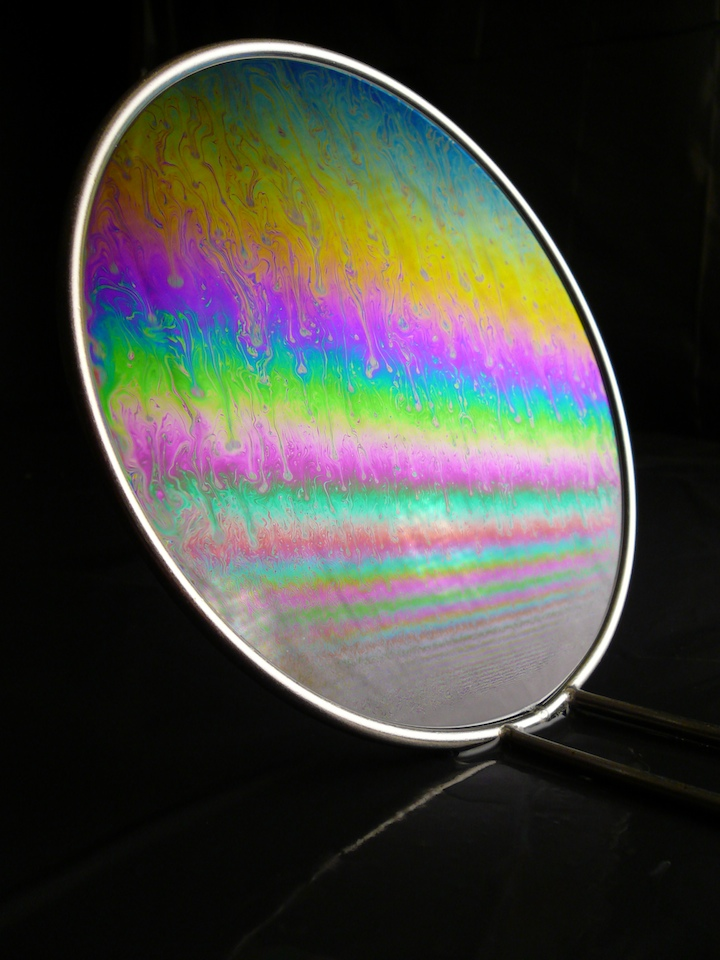
\includegraphics[height=5cm]{pic19.jpg}
\caption{Patr\'on de interferencia observado en pel\'\i culas delgadas
formadas por pompas de jab\'on.}
\label{fig:pompasjabon}
\end{figure}

La interferencia producida por pel\'\i culas delgadas fue observada por primera
vez por Isaac Newton y Robert Hooke. No obstante, la explicaci\'on correcta de
este fen\'omeno fue dada reci\'en varios a\~nos despu\'es por Thomas Young.

\section{Pel\'\i cula delgada de caras plano-paralelas}

Vamos a considerar ahora una pel\'\i cula o l\'amina transparente de espesor
uniforme $d$, compuesta por dos interfaces paralelas (una superior y otra 
inferior), seg\'un se muestra en la Fig.~\ref{fig:lcp}. Supongamos que el 
\'\i ndice de refracci\'on del material que compone la l\'amina delgada 
es $n$. Asimismo, la pel\'\i cula se encuentra rodeada por un mismo medio, 
el aire de \'\i ndice de refracci\'on igual a la unidad. 
Imaginemos que una fuente monocrom\'atica (de una \'unica longitud
de onda o {\it color}) extensa ilumina a la pel\'\i cula en forma obl\'\i cua.
Una onda plana monocrom\'atica, que puede considerarse como un haz paralelo, 
incide entonces sobre la superficie superior de la l\'amina. En el esquema,
el segmento $AB$ representa a uno de estos rayos incidentes.

\begin{figure}[ht]
    \centering
    \begin{overpic}[scale=0.4, unit=1mm]%
        {lamina.png}
        \put(75,40){$d$}
        \put(20,40){$n$}
        \put(5,60){salto de $\pi$}
        \put(55,37.5){sin salto}
        \put(70,57){aire}
        \put(70,25){aire}
    \end{overpic}
    \caption{Esquema empleado para derivar la diferencia de fase entre rayos
    para una l\'amina delgada de caras paralelas por reflexi\'on.}
    \label{fig:lcp}
\end{figure}




El rayo $AB$ se refleja parcialmente dando lugar al rayo $BC$, al tiempo que
se transmite parcialmente en el interior de la l\'amina a lo largo de $BF$.
Este rayo transmitido $BF$ forma un \'angulo $\theta_r$ con la normal a la
superficie inferior. En el punto marcado como $F$ en la figura, $BF$ se 
refleja parcialmente hacia la pel\'\i cula, sobre $FD$, mientras que una 
porci\'on mayor se refracta hacia el medio exterior a lo largo de $FK$. 
El rayo reflejado $FD$ luego se refracta en la superficie externa y emerge
de la l\'amina sobre $DE$, que es paralelo al rayo $BC$. De esta forma, las
ondas que viajan en las direcciones $BC$ y $BFDE$ se obtienen de la onda
incidente original, $AB$. Por esta raz\'on, ambas son coherentes entre s\'\i\
y pueden producir interferencia si se las hace converger, ya sea utilizando
una lente o el ojo. Como sabemos, la condici\'on de interferencia 
(constructiva o destructiva) depende de la diferencia de camino \'optico entre 
los rayos 1 y 2. 

Calculemos la diferencia de camino \'optico entre el rayo reflejado $BC$ 
(rayo 1) y el refractado $BFDE$ (rayo 2). La linea $DH$ es normal al segmento 
$BC$ y pasa por el punto $D$. A partir de la posici\'on de los puntos $H$ y $D$
los rayos  $HC$ y $DE$ viajan distancias iguales. El rayo reflejado $BC$ viaja
en aire, mientras que el refractado $(BF + FD)$ viaja en la l\'amina de 
\'\i ndice $n$. La diferencia de camino geom\'etrica (no \'optica) entre los
rayos 1 y 2 viene dada por:
\begin{equation}
GPD = BF + FD - BH.
\end{equation}
La diferencia de camino \'optico resulta entonces
\begin{equation}
    \Delta = n_\text{l\'amina} (BF+FD) - n_\text{aire} BH = n (BF+FD) - BH.
\end{equation}
Ahora bien, consideremos el tri\'angulo de v\'ertices $BFD$. En \'el, el 
\'angulo $BFG$ coincide con el \'angulo $GFD$, y es igual al \'angulo reflejado
$\theta_r$. Por otro lado, vemos que $BF = FD$ y $BG = GD$. De estos dos pares
de segmentos, el primero de ellos tiene una longitud dada por
\begin{equation}
    BF = \frac{FG}{\cos \theta_r} = \frac{d}{\cos \theta_r},
\end{equation}
por lo que podemos concluir que
\begin{equation}
    BF + FD = \frac{2d}{\cos \theta_r}.
\end{equation}
De manera similar, en f\'acil obtener 
\begin{equation}
BG = FG \tan \theta_r = d \tan \theta_r.
\end{equation}

Por otro lado, consideremos ahora el tri\'angulo de v\'ertices $BHD$. El 
\'angulo $HBD$ es de $(\pi/2 - \theta_i)$, mientras que el \'angulo $BHD$ es
de $\pi/2$ radianes. Esto permite deducir que el \'angulo $BDH$ es $\theta_i$.
Por lo tanto, la longitud del segmento $BH$ que buscamos viene dado por
\begin{equation}
BH = BD \sin \theta_i = 2 BG \sin \theta_i = 2 d \tan \theta_r \sin \theta_i.
\end{equation}
A partir de la ley de Snell, $\sin \theta_i = n \sin \theta_r$, por lo que
la \'ultima expresi\'on puede reducirse a
\begin{equation}
    BH = 2d \tan \theta_r \left( n \sin \theta_r \right) = 
    \frac{2 n d \sin^2 \theta_r}{\cos \theta_r}.
\end{equation}

A partir de estas derivaciones, la diferencia de camino \'optico entre los
rayos 1 y 2 resulta:
\begin{equation*}
    \Delta = n \left( \frac{2d}{\cos \theta_r} \right) - 2 n d 
    \frac{\sin^2 \theta_r}{\cos \theta_r} = \frac{}{} \left( 1 - \sin^2 
    \theta_r \right) = \frac{2nd \cos^2 \theta_r}{\cos \theta_r},
\end{equation*}
por lo que
\begin{equation}
\Delta = 2 n d \cos \theta_r. 
\end{equation}

Observemos que $\Delta$ es la diferencia de camino \'optico entre ambos rayos.
Deteng\'amonos un momento para preguntarnos: ?`qu\'e dimensiones tiene la
diferencia de camino \'optico? M\'as a\'un: dado que la diferencia de camino
\'optico est\'a definida como la diferencia entre las longitudes de camino
\'optico de dos caminos dados, ?`qu\'e unidades tiene la longitud de camino
\'optico?

En general, una longitud de camino \'optico es simplemente la longitud de un
camino en el espacio (una distancia) multiplicada por el 
\'\i ndice de refracci\'on del medio en el cu\'al est\'a inmerso dicho camino.
Siendo que el \'\i ndice de refracci\'on es una cantidad sin dimensiones 
(sin unidades), surge entonces que la longitud de camino \'optico tiene 
dimensiones de longitud, por lo que {\it la diferencia de camino \'optico 
entre dos rayos cualesquiera tiene dimensiones de longitud}. 

Multipliquemos entonces la \'ultima expresi\'on por el n\'umero de onda, $k$,
para obtener la diferencia de fase $\delta'$ entre ambos rayos:
\begin{equation}
    \delta' = k \cdot \Delta = k \cdot 2 n d \cos \theta_r = 2 n k d  
    \cos \theta_r.
\end{equation}
Notemos que la diferencia de fase entre los rayos 1 y 2 dada por
esta expresi\'on no es la diferencia de fase {\it total} entre ambos rayos, 
ya que {\it todav\'\i a resta considerar la diferencia de fase debida a la 
reflexi\'on}. En el punto $B$, ocurre una reflexi\'on desde la interfaz entre
el medio exterior a otro \'opticamente m\'as denso (de mayor \'\i ndice de 
refracci\'on), lo que resulta en un salto abrupto de $\pi$ radianes en la 
fase de la onda $BC$. 

Incluyendo entonces el salto de $\pi$ radianes, la diferencia de fase entre 
los rayos 1 y 2 resulta:
\begin{equation}
\delta = \delta' + \pi = 2 n k d \cos \theta_r + \pi.
\end{equation}
Ahora que tenemos la diferencia de fase entre ambos rayos, sabemos que la
intensidad o irradiancia del patr\'on de interferencia asociado ser\'a de 
la forma 
\begin{equation}
    I = I_0 \cos^2 (\delta/2),
\end{equation}
siendo $I_0$ una intensidad de referencia. En base a esta forma funcional, 
podemos entonces buscar la condici\'on para observar m\'aximos de intensidad, 
los cuales ocurrir\'an cuando
\begin{equation*}
    \cos (\delta/2) = 1,
\end{equation*}
es decir para 
\begin{equation*}
    \delta/2 = 0, \pm \pi, \pm 2\pi, \ldots, m \pi \quad \text{con} \quad
    m \in \Z_0. 
\end{equation*}

En t\'erminos de los par\'ametros del sistema f\'\i sico que tenemos, esta
condici\'on implica
\begin{equation*}
2 n k d \cos \theta_r + \pi = 2 m \pi, 
\end{equation*}
expresi\'on que puede reescribirse como
\begin{equation}
    2 n d \cos \theta_r = \left( 2 m + 1 \right) \frac{\lambda}{2}, \quad
    \quad m \in \Z_0,
\end{equation}
y representa la condici\'on para obtener un m\'aximo en el patr\'on de 
interferencia asociado. En este caso el valor de $m$ corresponde al {\it
orden} del m\'aximo de interferencia.

La condici\'on para obtener m\'\i nimos (ceros) de intensidad se obtiene en 
forma an\'aloga, y resulta:
\begin{equation}
    2 n d \cos \theta_r = m \lambda, \quad \quad m \in \Z_0,
\end{equation}
siendo ahora $m$ el orden del m\'\i nimo de interferencia.

Cada uno de los rayos que inciden sobre la l\'amina con el mismo \'angulo son 
divididos en dos, los cuales devienen paralelos luego de la reflexi\'on en 
las superficies (superior e inferior) de la pel\'\i cula. Estos rayos paralelos
no se intersectan a distancias finitas, por lo que la interferencia no se 
produce a distancias finitas tampoco. Para ello es necesario hacerlos incidir
sobre una lente convergente, y la interferencia puede observarse en el plano
focal de la misma. Alternativamente, el patr\'on puede verse empleando el 
ojo acomodado al infinito (haciendo foco en el infinito). En vista de esto,
decimos que este tipo de franjas de interferencia est\'an {\it localizadas
en el infinito}.

\subsection{Puntos importantes a tener en cuenta}

\subsubsection{Patr\'on al observar la l\'amina por transmisi\'on}

Al observar la l\'amina {\it desde abajo}, es decir, los rayos que se 
transmiten a trav\'es de ella, el patr\'on de intensidad registrado es el
complementario del que calculamos; por lo que las condiciones son ahora:
\begin{align}
    2 n d \cos \theta_r &= (2 m + 1) \frac{\lambda}{2}, 
    &&\text{para m\'\i nimos por transmisi\'on, y} \\
    2 n d \cos \theta_r &= m \lambda, 
    &&\text{para m\'aximos por transmisi\'on.}
\end{align}


\subsubsection{L\'amina de espesor infinitesimal}

Si la l\'amina tiene un espesor extremadamente bajo, tal que $d \ll \lambda$,
resulta f\'acil ver que la diferencia de fase $\delta$ resulta
\begin{equation}
    \delta = 2 n k d \cos \theta_r + \pi = 4 \pi n \frac{d}{\lambda} + \pi 
    \approx  \pi,
\end{equation}
por lo que la pel\'\i cula aparece completamente oscura cuando se observa 
la luz por ella reflejada (es decir, cuando se la observa 
{\it en reflexi\'on}). 

\subsubsection{En incidencia normal}

Cuando se emplea luz monocrom\'atica y se incide en forma normal sobre la
pel\'\i cula, $\theta_r = 0$ por lo que $\cos \theta_r = 1$. Esto da lugar
a las siguientes condiciones para m\'aximos y m\'\i nimos de intensidades:
\begin{align}
    2 n d &= (2 m + 1) \frac{\lambda}{2}, &&\text{para m\'aximos, y} \\
    2 n d &= m \lambda, &&\text{para m\'\i nimos.}
\end{align}

Observemos que la primera de estas dos ecuaciones implica que la l\'amina
parecer\'a brillante en luz reflejada cuando su espesor sea de $\lambda/4n$,
$3 \lambda/4n, 5\lambda/4n, \ldots$; y se ver\'a completamente oscura 
(en reflexi\'on) cuando su espesor sea de $\lambda/2n, \lambda/n, 3\lambda/2n,
\cdots$, etc. 

\subsubsection{Luz incidente monocrom\'atica y paralela}

Si la luz incidente es monocrom\'atica y paralela (por ejemplo, por que la
fuente que la genera se encuentra infinitamente distante de la l\'amina), 
entonces toda la l\'amina se ver\'a uniformemente brillante u oscura, dado
que el espesor d y el \'angulo de refracci\'on $\theta_r$ ser\'an, entonces,
constantes. La condici\'on para interferencia constructiva causa entonces
una intensificaci\'on del color incidente en este caso. Luego si se incide
con luz roja sobre la pel\'\i cula, una luz intensa y roja ser\'a observada
en luz reflejada.

\subsubsection{El rol del \'angulo de incidencia}

Un cambio en el \'angulo de incidencia de los rayos causar\'a un cambio en la
diferencia de camino y, por ende, en la diferencia de fase. Observemos que la 
diferencia de camino \'optico se reduce cuando el \'angulo de incidencia 
aumenta.

\subsubsection{Incidencia con luz blanca}

Si luz blanca incide ahora sobre la pel\'\i cula, la diferencia de camino
\'optico (y de fase) variar\'a de un color a otro, dado que $\lambda$ es
distinta para colores distintos. De acuerdo a esto, la pel\'\i cula aparecer\'a
coloreada, el color observado corresponder\'a a aquel cuyos rayos hayan 
interferido constructivamente. M\'as a\'un, el color de la l\'amina toda 
cambiar\'a a medida que su inclinaci\'on sea variada.

\subsection{El rol del espesor de la pel\'\i cula}

De acuerdo a lo calculado hasta ahora, podr\'\i amos pensar que toda l\'amina
de caras paralelas es capaz de generar patrones de interferencia. No obstante,
la experiencia cotidiana nos dice que, si bien es posible observar estos 
patrones en l\'aminas delgadas (burbujas de jab\'on), los mismos no parecen
producirse en pel\'\i culas m\'as gruesas, tales como 
las formadas por los vidrios de los que est\'an hechas nuestras ventanas. 
?`Qu\'e es lo que impide o restringe la generaci\'on de patrones de 
interferencia en estos casos?

Seg\'un vimos en clase, una condici\'on fundamental para que dos haces de luz 
interfieran es que sean coherentes. As\'\i\ , cuando el espesor de la 
pel\'\i cula es menor que la longitud de coherencia de las ondas incidentes,
es posible observar interferencia. En l\'aminas gruesas no observamos 
interferencia ya que los haces pierden coherencia. 

% \subsection{Una aplicaci\'on importante: recubrimientos antireflectivos}

% Imaginemos ahora que buscamos reducir la reflectividad de una superficie 
% \'optica dada, por ejemplo la de los cristales de nuestros anteojos. Para ello,
% depositamos sobre los cristales una capa delgada de alg\'un material
% transparente (que 
% har\'a las veces de l\'amina de caras paralelas en contacto con el vidrio de 
% nuestros anteojos). 

% Nuestros resultados precedentes nos dicen que si elegimos correctamente el 
% espesor de la capa con la que recubrimos nuestros cristales, es posible
% que la l\'amina de caras paralelas as\'\i\   dispuesta genere interferencia
% destructiva entre las ondas reflejadas en las caras frontal y trasera de 
% dicha pel\'\i cula. Esta es la idea de base detr\'as de lo que hoy conocemos
% como {\it recubrimientos antireflectivos}. Estos recubrimientos fueron inventados 
% por Olexander Smakula (1900-1983) en el a\~no 1935 mientras que Smakula trabajaba para Zeiss. 

% Supongamos que luz monocrom\'atica incide normalmente sobre este recubrimiento
% en nuestros anteojos. La incidencia normal hace que $\theta \approx 0$, con 
% lo cu\'al $\cos \theta \approx 1$.  





La interferencia resultante de la luz reflejada en una l\'amina de caras
paralelas dispuesta sobre otra superficie transparente puede emplearse para
reducir la reflectividad el sustrato sobre el cu\'al yace dicha capa. 



\section{Pel\'\i cula de espesor variable o cu\~na}

\begin{figure}
    \centering
    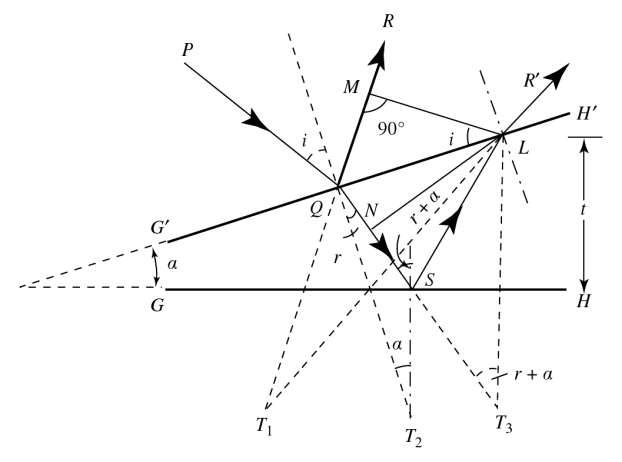
\includegraphics[scale=0.5]{wedge.png}
    \label{fig:cuna}
    \caption{Esquema empleado para derivar la diferencia de camino entre rayos
        en una cu\~na.}
\end{figure}
Vamos a estudiar ahora la interferencia producida por una pel\'\i cula o 
l\'amina de espesor variable. Este caso se denomina tambi\'en cu\~na (`wedge'
en ingl\'es). 

Consideraremos una cu\~na como la que se muestra esquem\'aticamente en la
Fig.~\ref{fig:cuna}. La misma se define como una pel\'\i cula de espesor
variable, encerrada entre dos caras planas, dadas por $GH$ y $G'H'$, inclinadas
una respecto de la otra en un \'angulo $\alpha$. Para hacerlo m\'as concreto,
asumiremos que el espesor de la l\'amina aumenta de $G$ a $H$, y que el 
\'\i ndice de refraccion de la pel\'\i cula viene dado por $n$. Vamos a suponer
adem\'as que iluminamos la cu\~na con luz monocrom\'atica. 

En este caso la interferencia es producida por dos rayos: uno es el reflejado 
por la superficie frontal de la pel\'\i cula en forma de cu\~na, y el segundo 
corresponde a la reflexi\'on interna en la superficie inferior, que luego
es transmitido hacia fuera por la interfaz superior. Las dos ondas que dan
lugar a interferencia, denotadas en la figura por $QR$ y $LR'$ no son paralelas
sino que parecen diverger de un punto com\'un, $T_1$. Esto significa que en
el punto $T_1$ tiene lugar lo que denominamos una {\it interferencia virtual}.

A fin de analizar la interferencia en ese punto, debemos calcular la diferencia
de camino \'optico entre ambas ondas. La misma puede escribirse como
\begin{align*}
    \Delta &= n \left( QS + SL \right) - QM \\
           &= n \left( QN + NS + SL \right) - n \cdot QN \\
           &= n \left( NS + SL \right) \\
           &= n \cdot NT_3,
\end{align*}
para finalmente obtener
\begin{equation}
    \Delta = 2 n d \cos \left( \theta_r + \alpha \right).
\end{equation}
La diferencia de fase asociada a esta diferencia de camino la obtenemos de
\begin{equation}
    \delta' = 2 n k d \cos \left( \theta_r + \alpha \right).
\end{equation}
Finalmente, a esta diferencia de fase vinculada con la diferencia de camino
debemos agregarle la diferencia de fase de $\pi$ radianes debida a la 
reflexi\'on en el interior de la cu\~na. La diferencia de fase
total, $\delta$, resulta
\begin{equation}
    \delta = 2 n k d \cos \left( \theta_r + \alpha \right) + \pi.
\end{equation}

A partir de esta diferencia de fase resulta inmediato calcular las condiciones
para obtener m\'aximos y m\'\i nimos {\bf de reflexi\'on}, que vienen dados 
por: 
\begin{align}
    2 n d \cos \left( \theta_r + \alpha \right) &= \left( 2 m + 1 \right) 
    \frac{\lambda}{2}, \quad &&m \in \Z_0, \quad \quad \text{para m\'aximos, y}
    \\
    2 n d \cos \left( \theta_r + \alpha \right) &= m \lambda, \quad &&m \in 
    \Z_0, \quad \quad \text{para m\'\i nimos}.
\end{align}

\subsection{Puntos importantes a tener en cuenta}

\subsubsection{Acerca del patr\'on de interferencia}

Consideremos un haz monocrom\'atico y paralelo de longitud de onda $\lambda$
que incide sobre la cu\~na. El \'angulo de incidencia, y por ende el \'angulo
de refracci\'on $\theta_r$ son constantes sobre toda la cu\~na. Por otro lado,
tambi\'en son constantes el \'angulo $\alpha$ y el \'\i ndice de refracci\'on
que caracterizan a la cu\~na. De esta forma, el espesor {\it local} de la 
pel\'\i cula es el factor determinante para la diferencia de fase que
calculamos; luego si una franja es brillante u oscura debido a interferencia
depende de $d$, que es constante sobre toda l\'\i nea paralela al v\'ertice
de la cu\~na. Por lo tanto, el patr\'on de interferencia (de observarse uno)
consiste de franjas rectas paralelas al borde de la cu\~na. Franjas brillantes
u oscuras se obtienen de acuerdo al valor del espesor local $d$ y las \'ultimas
condiciones que derivamos.

\subsubsection{La franja ubicada en el \'apice de la cu\~na es oscura}

En el \'apice, el espesor de la cu\~na es muy peque\~no en comparaci\'on a
la longitud de onda de la luz incidente, $\lambda$, es decir $d \ll \lambda$.
Por ende la diferencia de fase en ese lugar es igual a $\pi$ radianes. Esto
implica que los rayos que interfieren siempre estar\'an en contrafase, 
interfiriendo destructivamente en el \'apice. Por lo tanto, el patr\'on de
interferencia de la cu\~na comenzar\'a siempre con una franja oscura.

\subsubsection{Franjas de espesor constante}

Dado que cada m\'aximo o m\'\i nimo ocurre en puntos donde el espesor de la
pel\'\i cula es constante, a este tipo de franjas de interferencia se las
denomina franjas de espesor constante.

\subsubsection{Ancho de las franjas}

Para el m\'aximo $n$-\'esimo, la condici\'on es
\begin{equation}
    2 n d \cos \left( \theta_r + \alpha \right) = \left( 2 m + 1 \right) 
    \frac{\lambda}{2}.
\end{equation}
Si estamos considerando una pel\'\i cula de aire y en incidencia normal,
tenemos $n = 1$ y $\theta_r = 0$. Luego la condici\'on de m\'aximo se 
reduce a
\begin{equation}
    2 d \cos \left( \alpha \right) = \left( 2 m + 1 \right) 
    \frac{\lambda}{2}.
\end{equation}

Supongamos que ese mismo m\'aximo $n$-\'esimo ocurre a una distancia $x_n$
medida desde el v\'ertice de la cu\~na en la direcci\'on horizontal, donde
el espesor local es $d_n$. A partir de esto tenemos
\begin{equation}
    d = x_n \tan \alpha,
\end{equation}
por lo que 
\begin{equation*}
    2 x_n \tan \alpha \cos \alpha = (2m+1) \frac{\lambda}{2},
\end{equation*}
es decir que
\begin{equation*}
    2 x_n \sin \alpha = (2 m +1 ) \frac{\lambda}{2}.
\end{equation*}
Ahora bien, el siguiente m\'aximo, el $(n+1)$-\'esimo se ubicar\'a a una 
distancia $x_{n+1}$, luego
\begin{equation*}
    2 x_{n+1} \sin \alpha = (2m +3) \frac{\lambda}{2}.
\end{equation*}

El ancho de la franja viene entonces dado por la distancia entre las dos 
franjas consecutivas, la $(n+1)$ y la $n$. Esa diferencia es
\begin{equation}
    2 \left( x_{n+1} - x_n \right) \sin \alpha = \left( 2m + 3 - 2m -1\right)
    \frac{\lambda}{2} = \lambda,
\end{equation}
por lo que el ancho de las franjas, que denominaremos $\gamma$ resulta
\begin{equation}
    \gamma = x_{n+1} - x_n = \frac{\lambda}{2 \sin \alpha}.
\end{equation}
M\'as a\'un, si la cu\~na es de \'angulo peque\~no, $\sin \alpha \approx 
\alpha$, por lo que el ancho resulta
\begin{equation}
    \gamma = \frac{\lambda}{2\alpha}, \quad \text{(con $\alpha$ en radianes)}.
\end{equation}
En raz\'on de este resultado, decimos que las franjas de interferencia en 
este caso son de ancho constante. Notemos que si el \'\i ndice de refracci\'on
de la pel\'\i cula fuese $n$, este resultado se generaliza f\'acilmente a
\begin{equation}
    \gamma = \frac{\lambda}{2 n \alpha}.
\end{equation}

% \subsubsection{Espesor de elemento que separa la cu\~na}

% Asumamos que la cu\~na se forma introduciendo un objeto (podr\'\i a ser una
% fibra delgada o un pelo) a una distancia $L$ del v\'ertice de la cu\~na. A 
% este objeto se lo denomina usualmente {\it espaciador}. Lo interesante en 
% este punto es que podemos determinar el espesor del espaciador a partir de la
% observaci\'on del patr\'on de interferencia empleando las relaciones que 
% derivamos en las secciones precedentes. El espesor $d$ ser\'a entonces
% \begin{equation}
% d = L \tan \alpha \approx L \alpha,
% \end{equation}
% donde hemos supuesto que el \'angulo de la cu\~na es peque\~no ($\alpha \ll 1$)
% de forma de poder aproximar la tangente por el \'angulo mismo. 

\section{Anillos de Newton}

Otro ejemplo cl\'asico de franjas de igual espesor son los denominados
anillos de Newton. Los mismos se observan cuando la luz se refleja en una
lente plano-convexa de gran distancia focal dispuesta sobre una l\'amina 
de caras paralelas, seg\'un se muestra esquem\'aticamente en la 
Fig.~\ref{fig:anillos}. La capa de aire entre ambas piezas 
\'opticas juega aqu\'\i\ el rol de pel\'\i cula delgada. El espesor de esta
pel\'\i cula es cero en el punto de contacto entre ambas piezas. Si este 
sistema es iluminado con luz monocrom\'atica en incidencia normal a la 
superficie plana de la lente, es posible observar (por reflexi\'on) un patr\'on
de interferencia compuesto de anillos conc\'entricos alternadamente brillantes 
y oscuros. Estas franjas fueron descubiertas por Isaac Newton, raz\'on por la
cu\'al llevan su nombre. No obstante, fue Thomas Young qui\'en di\'o la 
explicaci\'on acerca de su formaci\'on.  

\begin{figure}[ht]
\centering
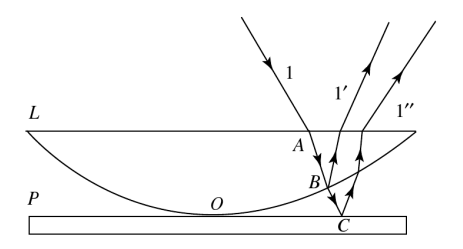
\includegraphics[height=5cm]{anillos.png}
\caption{Esquema para el an\'alisis de la interferencia (por reflexi\'on)
en anillos de Newton.}
\label{fig:anillos}
\end{figure}

Cuando el rayo $1$ incide sobre el sistema, el mismo se refleja parcialmente 
en la superficie curvada inferior de la lente (punto $B$) y luego una parte del rayo 
transmitido se refleja parcialmente  desde la superficie superior de la 
l\'amina de caras paralelas (punto $C$). De esta forma, los rayos $1'$ y $1''$ se derivan
del mismo rayo incidente por divisi\'on de amplitud, y son por lo tanto 
coherentes entre s\'\i . El primero de estos rayos no sufre cambio de fase
por reflexi\'on, pero s\'\i\   el segundo. En particular, el rayo $1''$ 
experimenta un salto de $\pi$ radianes al reflejarse en la interfaz aire-vidrio
correspondiente a la superficie superior de la l\'amina de caras paralelas. 
Cabe destacar, adem\'as, que no se observa interferencia entre los rayos 
reflejados en las superficies de la lente y de la l\'amina de caras paralelas
(no representados en la Fig.~\ref{fig:anillos}) debido a sus espesores. 

En consecuencia, las condiciones para interferencia constructiva y destructiva
para los rayos $1'$ y $1''$ est\'an dadas por
\begin{align}
    2 n d \cos \left( \theta_r \right) &= \left( 2 m + 1 \right) 
    \frac{\lambda}{2}, \quad &&m \in \Z_0, \quad \quad \text{para m\'aximos, y}
    \\
    2 n d \cos \left( \theta_r \right) &= m \lambda, \quad &&m \in 
    \Z_0, \quad \quad \text{para m\'\i nimos}.
\end{align}
Nuevamente, en el caso particular de incidencia normal (que es frecuente cuando
se observan anillos de Newton), tenemos que $\cos \theta_r = 1$, luego
\begin{align}
    2 n d &= \left( 2 m + 1 \right) 
    \frac{\lambda}{2}, \quad &&m \in \Z_0, \quad \quad \text{para m\'aximos, y}
    \\
    2 n d &= m \lambda, \quad &&m \in 
    \Z_0, \quad \quad \text{para m\'\i nimos},
    \label{eq:fet}
\end{align}
siempre para el caso de las franjas observadas {\it en reflexi\'on}.

\subsection{Puntos importantes a tener en cuenta}

\subsubsection{Spot central oscuro}

En el punto de contacto entre la lente plano-convexa y la l\'amina de caras
paralelas, el espesor de la pel\'\i cula de aire es de s\'olo algunas 
mol\'eculas, es decir, muy peque\~na en comparaci\'on con la longitud de onda
($d_\text{centro} \ll \lambda$). La diferencia de camino introducida entre las
ondas que interfieren en ese punto es entonces nula, luego $2 d = 0$ 
localmente. Sin embargo, debido a la reflexi\'on, la onda reflejada en la 
superficie superior de la l\'amina de caras paralelas sufre un cambio de fase
de $\pi$ radianes. Consecuentemente, las ondas que interfieren en el centro
del sistema est\'an en contrafase e interfieren destructivamente all\'\i .

De esta forma, en el \'area de contacto entre la lente y el plano, se observa
un spot oscuro. Esta es una evidencia directa del cambio de fase relativo
(de $\pi$ radianes) entre los dos tipos de reflexiones: aire-vidrio y 
vidrio-aire. 

\subsubsection{Franjas de espesor constante}

A partir de las ecuaciones \eqref{eq:fet} puede verse que la aparici\'on de
m\'aximos y m\'\i nimos se debe a la variaci\'on local del espesor de la 
pel\'\i cula de aire, $d$. Cada m\'aximo o m\'\i nimo corresponde a puntos
donde la pel\'\i cula de aire tiene un mismo valor de espesor. Por esta raz\'on
estas franjas son tambi\'en {\it franjas de espesor constante}. 

\subsubsection{Franjas circulares}

Esta l\'amina de aire de espesor variable puede pensarse como una cu\~na rotada
alrededor del punto de contacto. El conjunto de puntos que presenta igual 
espesor yace entonces sobre un c\'\i rculo que tiene su centro en el punto
de contacto entre las dos piezas \'opticas que delimitan la pel\'\i cula de 
aire. En consecuencia, el espesor de dicha pel\'\i cula es el mismo en todos
los puntos sobre cualquier c\'\i rculo que tiene a dicho punto como centro. 
Las franjas son entonces circulares.

\subsubsection{Franjas localizadas}

Cuando el sistema es iluminado por luz paralela, los rayos reflejados no son
paralelos. Dichos rayos interfieren cerca de la superficie superior de la 
pel\'\i cula de aire y parecen diverger a partir de all\'\i   cuando se los 
observa desde arriba. En este caso, las franjas se observan cerca de la
superficie superior de la pel\'\i cula y, por tanto, se dice que est\'an 
localizadas sobre la pel\'\i cula.

\subsubsection{Radio de los anillos oscuros}

Vamos ahora a calcular el radio de los anillos oscuros correspondientes al
patr\'on de interferencia; para ello emplearemos el esquema de la 
Fig.~\ref{fig:anillos2}.

\begin{figure}[ht]
\centering
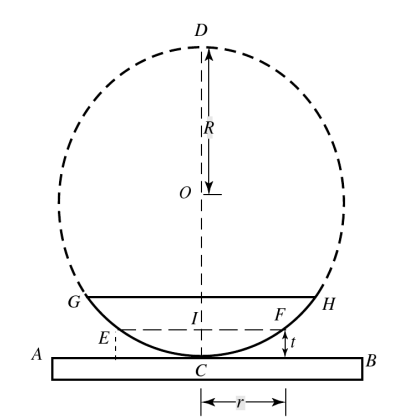
\includegraphics[height=6cm]{anillos2.png}
\caption{Esquema para determinar el radio de los anillos oscuros.}
\label{fig:anillos2}
\end{figure}

Sea entonces $R$ el radio de curvatura de la lente plano-convexa. Consideremos
adem\'as un anillo ubicado en un punto $r$. El espesor de la 
pel\'\i cula de aire en ese punto es $t$. Identifiquemos con $r_m$ a la 
posici\'on radial del $m$-\'esimo anillo. Del diagrama vemos que
\begin{equation*}
IF \cdot IE = IC \cdot ID.
\end{equation*}
A partir de la geometr\'\i a de la Fig.~\ref{fig:anillos}, es posible 
hacer las siguientes identificaciones
\begin{align*}
    IF &= r_m, \\
    IE &= r_m, \\
    IC &= t, \\ 
    ID &= 2R - t.
\end{align*}
Sustituyendo ahora estas cuatro identificaciones en la igualdad precedente,
obtenemos
\begin{equation*}
r_m \cdot r_m = t \cdot (2R - t), 
\end{equation*}
por lo que 
\begin{equation*}
r_m^2 = 2Rt - t^2.
\end{equation*}
Ahora bien, si $t$ es muy peque\~no comparado con $R$, podemos entonces
despreciar $t^2$ frente a $2Rt$, para obtener:
\begin{equation*}
    r_m^2 \approx 2 R t.
\end{equation*}

Usando ahora la condici\'on de m\'\i nimo de intensidad en este punto de 
espesor $t$,
\begin{equation*}
    2 n t = m \lambda, \quad \text{con $m \in \Z_0$}, 
\end{equation*}
tenemos
\begin{equation*}
r_m^2 = m \lambda R,
\end{equation*}
es decir que el radio del $m$-\'esimo anillo oscuro viene dado por
\begin{equation}
    r_m^\text{osc} = \sqrt{m \lambda R}.
\end{equation}

El radio de los diferentes anillos oscuros puede hallarse sustituyendo en
$m$ los n\'umeros naturales, incluido el cero. Se observa entonces que la 
progresi\'on de radios oscuros viene dada por:
\begin{align*}
    r^\text{osc}_0 &= 0, \\
    r^\text{osc}_1 &= \sqrt{\lambda R}, \\
    r^\text{osc}_2 &= \sqrt{2} \sqrt{\lambda R}, \\
    r^\text{osc}_3 &= \sqrt{3} \sqrt{\lambda R}, \\
    r^\text{osc}_4 &= \sqrt{4} \sqrt{\lambda R}, \\
    \text{etc.}
\end{align*}
Es decir que los radios (y tambi\'en los di\'ametros) de los anillos de 
Newton oscuros son proporcionales a la ra\'\i z cuadrada de los n\'umeros
naturales.

\subsubsection{Radio de los anillos brillantes}

Empleando el mismo mecanismo que en la secci\'on precedente, es posible hallar
el radio de los anillos brillantes, utilizando ahora la condici\'on de m\'aximo
de intensidad en lugar de la de m\'\i nimo que usamos antes. Este c\'alculo
sencillo arroja que el radio del $m$-\'esimo anillo brillante viene dado por
\begin{equation}
    r^\text{bri}_m = \sqrt{\frac{2m+1}{2}} \sqrt{\lambda R}.
\end{equation}
De esto surge que los radios (y tambi\'en los di\'ametros) de los anillos
de Newton brillantes son proporcionales a la ra\'\i z cuadrada de los 
n\'umeros naturales {\it impares}. 

\subsubsection{El espaciado entre anillos se reduce conforme nos alejamos
del centro}

Vimos que los di\'ametros de los anillos oscuros son proporcionales a la 
ra\'\i z cuadrada de los n\'umeros naturales, mientras que los di\'ametros de 
los anillos brillantes son proporcionales a la ra\'\i z cuadrada de los 
n\'umeros naturales impares. A medida que el orden de los anillos se 
incrementa ($m$ aumenta), el di\'ametro no aumenta en la misma proporci\'on,
lo que resulta en que los anillos se acercan a medida que nos alejamos
del centro del sistema. 

\subsubsection{Patr\'on en luz transmitida}

Como es de esperar, tambi\'en se observa un patr\'on de interferencia en 
luz transmitida, es decir, mirando los rayos que se transmiten a trav\'es del
sistema. Estos anillos son exactamente complementarios a los observados por
reflexi\'on, por lo cu\'al el spot central en transmisi\'on es brillante. 

\subsubsection{Incidencia con luz blanca}

Si iluminamos al sistema con luz blanca, obtenemos una serie de anillos de
colores, dado que el radio de cada anillo depende de la longitud de onda
incidente, seg\'un vimos anteriormente.

\subsubsection{Determinaci\'on de la longitud de onda incidente}

Si sabemos que se incide con luz monocrom\'atica, pero desconocemos su longitud
de onda; es posible determinar esta \'ultima a partir del examen del patr\'on
de interferencia. Consideramos entonces el $m$-\'esimo anillo oscuro, cuyo
di\'ametro podemos medir y deber\'\i a estar dado por
\begin{equation}
    D_m^\text{osc} = 4 m \lambda R.
\end{equation}
Luego buscamos el $(m+p)$-\'esimo anillo oscuro, cuyo di\'ametro es
\begin{equation}
    D_{m+p}^\text{osc} = 4 (m+p) \lambda R.
\end{equation}
A partir de estas dos expresiones resulta f\'acil obtener la longitud de 
onda buscada:
\begin{equation}
    \lambda = \frac{\left(D_{m+p}^\text{osc}\right)^2 - 
    \left(D_{m}^\text{osc}\right)^2}{4 p R}.
\end{equation}
Obs\'ervese que esta expresi\'on depende del radio de curvatura $R$ de la lente
plano-convexa. En la pr\'actica, el mismo puede medirse empleando un 
esfer\'ometro.


\section*{Referencias}
\begin{itemize}
    \item Optics. E. Hecht. Addison-Wesley (2001).
    \item Modern Optics. R. Guenther. Wiley (1990). 
\end{itemize}

\end{document}
